\documentclass[conference]{IEEEtran}

\usepackage{amsmath,amssymb}
\usepackage{booktabs}
\usepackage{graphicx}
\usepackage{url}

\title{Evolving Zero-Float Q7 Autonomous Policies for a 16-Bit FRAM Microcontroller Roguelike}

\author{\IEEEauthorblockN{joaogpd}
\IEEEauthorblockA{\textit{mspgame Embedded Systems Project} \\
TI MSP430FR5994 LaunchPad Platform}}

\begin{document}

\maketitle

\begin{abstract}
Deploying autonomous game-playing agents on ultra-low-power 16-bit microcontrollers without a hardware Floating-Point Unit (FPU) requires compact policy representations, strict memory discipline, and bit-faithful offline-to-hardware transfer. We present an end-to-end evolutionary pipeline and on-chip deployment for \texttt{mspgame}, a procedural 80$\times$24 ANSI/VT100 roguelike running on the Texas Instruments MSP430FR5994 (16-bit core, 256~KB FRAM, 8~KB SRAM). We construct a bit-faithful Python headless simulator matching the firmware's 16-bit Galois LFSR (\texttt{0xB400}), 48$\times$22 dungeon tile layout, integer Bresenham line-of-sight, and combat rules, and evolve two zero-float Q7 \texttt{int8\_t} policy architectures: Approach~A, a 22-parameter action-conditioned linear heuristic (22~B in FRAM), and Approach~B, a 587-parameter fixed-topology Tiny-MLP (24$\rightarrow$16$\rightarrow$11 ReLU, 587~B in FRAM). Across a 12-experiment benchmark matrix (2,021.39~s total trainer wall-clock time) spanning compute budgets (Smoke, Medium, Deep), observability modes (Fair Fog-of-War vs.\ Omniscient), and three playable classes (Knight, Arcanist, Rogue), the 22-byte Heuristic~A outperforms the 587-byte Tiny-MLP~B by 1.36$\times$ to 10.95$\times$ on 10 unseen held-out seeds---reaching Floor~6 and defeating the Floor-5 Bone Warden boss under Fair Fog-of-War (3,156.7 mean held-out fitness)---while symmetric Q7 \texttt{int8\_t} quantization achieves 101.08\% mean (100.00\% median, 95.66\%--115.38\% range) fitness retention relative to Float32. Both models are compiled directly into the MSP430FR5994 firmware (609~B of FRAM weights, 3,668~B of inference code, 2,385/4,096~B total RAM, 45.7/262.0~KB total FRAM, 0~B dynamic heap), validated via live Hardware-in-the-Loop UART testing (\texttt{COM4 @ 115200} baud, 55 Heuristic~A turns and 34 Tiny-MLP~B turns, 0 deaths), and exposed interactively via an on-chip \texttt{[4] AI DEMO} mode supporting live Heuristic/MLP toggling.
\end{abstract}

\begin{IEEEkeywords}
Genetic Algorithms, TinyML, Q7 Fixed-Point Quantization, MSP430FR5994, FRAM, Embedded AI, Procedural Roguelike.
\end{IEEEkeywords}

\section{Introduction}
Embedded machine learning (TinyML) predominantly targets 32-bit Arm Cortex-M microcontrollers with DSP/SIMD extensions and tens to hundreds of kilobytes of SRAM. Ultra-low-power 16-bit microcontrollers such as the TI MSP430FR5994 operate under tighter constraints: no hardware FPU, 4~KB of general-purpose SRAM (\texttt{RAM}), and byte-addressed non-volatile Ferroelectric RAM (FRAM). Yet sequential decision-making tasks---such as navigating procedural dungeons under partial observability, resource management, and tactical combat---can be executed autonomously on-chip when policy representation, feature extraction, and fixed-point quantization are co-designed with the target hardware.

We investigate evolutionary policy optimization for \texttt{mspgame}, an ANSI/VT100 roguelike dungeon crawler written in C for the MSP430FR5994 LaunchPad. Using a parallel Genetic Algorithm (GA) over a bit-faithful offline simulator, we export symmetric Q7 \texttt{int8\_t} weights directly into FRAM \texttt{.const} arrays. Our contributions are:
\begin{enumerate}
    \item \textbf{Bit-Faithful Offline-to-MCU Parity:} A headless Python simulator (\texttt{ga/sim.py}) replicating the firmware's \texttt{0xB400} Galois LFSR, 48$\times$22 grid bitfields, three floor biomes, integer Bresenham line-of-sight (LOS), and 11-action combat/item mechanics.
    \item \textbf{Controlled 12-Experiment Benchmark:} An empirical comparison of a 22-parameter action-conditioned Heuristic (Approach~A) against a 587-parameter Tiny-MLP (Approach~B) across progressive compute tiers, Fair Fog-of-War vs.\ Omniscient perception, and three playable classes.
    \item \textbf{Zero-Float Q7 On-Chip Deployment:} A power-of-2 shift Q7 quantization scheme achieving 101.08\% mean retention across all 12 champions, deployed in 609~B of FRAM (0.23\% of device FRAM) with 0~B dynamic heap and validated live over \texttt{COM4 @ 115200} baud.
\end{enumerate}

\section{Target Hardware \& Game Environment}

\subsection{TI MSP430FR5994 Hardware Platform}
The target platform is the Texas Instruments \texttt{MSP-EXP430FR5994} LaunchPad featuring a 16-bit MSP430X CPU, a 32-bit hardware multiplier (\texttt{MPY32}), 256~KB FRAM (262,008 usable bytes across \texttt{FRAM} and \texttt{FRAM2}), 4~KB main SRAM (4,096~B), 4~KB Low-Energy Accelerator SRAM (\texttt{LEARAM} + \texttt{LEASTACK}, 4,096~B), and backchannel USB UART (\texttt{UART\_A0} at 115200~baud)~\cite{ti_ds,ti_ug}. Because software floating-point emulation incurs heavy code-size and cycle penalties on MSP430, all on-chip AI inference uses strictly signed 8-bit features/weights (\texttt{int8\_t}) and 32-bit integer accumulators (\texttt{int32\_t}).

\subsection{Procedural Roguelike Environment (\texttt{mspgame})}
The firmware renders an 80$\times$24 ANSI/VT100 terminal with a 28$\times$17 scrolling viewport over a 48$\times$22 (1,056-cell) dungeon map (1~B/cell: low 4 bits encode 13 tile types; high 4 bits encode \texttt{EXPLORED}, \texttt{VISIBLE}, \texttt{REVEALED}, and \texttt{ALT} flags). Procedural floors cycle across three biomes: \emph{Stone Crypt} (up to 8 non-overlapping rooms, L-shaped corridors with loops, up to 6 closed doors), \emph{Fungal Caverns} (420-step bounded random walk from $(24, 11)$), and \emph{Boss Sanctum} (every 5th floor, housing the Bone Warden boss with 24 base HP and 3~DMG).

Three playable classes provide distinct risk--reward trade-offs: \emph{Knight} (16~HP, 4~MP, 3~ATK, 1~DEF), \emph{Arcanist} (11~HP, 8~MP, 2~ATK, 0~DEF, piercing Arcane Bolt), and \emph{Rogue} (12~HP, 5~MP, 2~ATK, 0~DEF, 25~gold, $+1$ LOS radius 7 vs.\ 6, trap spot radius 4 vs.\ 2, $+2$ melee bonus vs.\ full-HP targets, starting Scroll of Mapping). Six enemy archetypes scale with floor depth. Each turn, the agent selects among 11 discrete actions: 4 cardinal moves/melee (\texttt{w,d,s,a}), 3 spells (\texttt{f} Arcane Bolt, \texttt{q} Frost Nova, \texttt{e} Blink), 3 items (\texttt{1} Potion, \texttt{2} Bomb, \texttt{3} Scroll of Mapping), or Focus/Wait (\texttt{' '}).

\section{Methodology}

\subsection{Bit-Faithful Headless Simulator}
\texttt{DungeonSim} (\texttt{ga/sim.py}) mirrors \texttt{app/dungeon\_game.c} down to the 16-bit Galois LFSR polynomial \texttt{0xB400} (default seed \texttt{0x5D17} $\rightarrow$ \texttt{0x9A8B}), integer Bresenham LOS~\cite{bresenham}, and combat/shop/trap rules. Episodes terminate on death, \texttt{max\_turns} $= 350$, or \texttt{stall\_turns} $= 140$ turns on one floor without descending.

\subsection{Perception, Observability Modes, and Action Masking}
Both policies share a single-pass, zero-allocation scanner (\texttt{precompute\_context}) using only Manhattan distances and cardinal raycasts (no BFS/A*). Under \textbf{Fair Fog-of-War}, only \texttt{EXPLORED} tiles and \texttt{VISIBLE} enemies are scanned; dormant mimics appear as chests, unrevealed traps appear as floor, and the scanner tracks the nearest unexplored frontier. Under \textbf{Omniscient} mode (ablation upper bound), the full 48$\times$22 map and all enemies/traps are visible. Pre-scoring action masking (\texttt{valid\_action\_mask}) eliminates illegal actions, yielding 0.0 wall bumps across all runs.

\subsection{Policy Architectures: Heuristic~A vs.\ Tiny-MLP~B}
All features are bounded in $[-1, 1]$ for Q7 quantization:
\begin{itemize}
    \item \textbf{Approach~A (\texttt{HeuristicGenome}, 22 params):} For each valid action $a \in \mathcal{V}(s)$, computes an action-conditioned vector $\phi(s, a) \in [-1, 1]^{22}$ (melee/kill, stairs/loot/shop/door/trap indicators, Manhattan step deltas toward stairs/loot/frontier/enemy, visit novelty, danger delta, bolt alignment, spell/item urgency, low-HP escape) and selects $a^* = \arg\max_{a \in \mathcal{V}(s)} w^\top \phi(s, a)$.
    \item \textbf{Approach~B (\texttt{TinyMLPGenome}, 587 params):} Computes a 24-element ego-state vector $x \in [-1, 1]^{24}$ (HP/MP ratios, empowerment, consumables, bolt target ahead, 4 cardinal neighbor encodings, 4 enemy raycasts, relative $(dx, dy)$ to stairs/frontier/loot/enemy, 3$\times$3 adjacent enemies, danger/boss flag) and evaluates a $24 \to 16 \to 11$ ReLU MLP ($24\cdot 16 + 16 + 16\cdot 11 + 11 = 587$ parameters):
    \begin{equation}
    \begin{aligned}
        h &= \operatorname{ReLU}(W_1 x + b_1), \quad z = W_2 h + b_2, \\
        a^* &= \arg\max_{a \in \mathcal{V}(s)} z_a.
    \end{aligned}
    \end{equation}
\end{itemize}

\subsection{Fitness Function \& Evolutionary Operators}
Episode fitness combines progression, exploration, combat, economy, and boss clears:
\begin{equation}
\begin{aligned}
F &= 500(\text{best\_floor} - 1) + 2\,\text{total\_explored} + 15\,\text{kills} \\
  &\quad + \text{gold} + 60\,\text{shops\_bought} + 1500\,\text{boss\_kills} \\
  &\quad - 0.5\,\text{wall\_bumps}.
\end{aligned}
\end{equation}
Genomes are evaluated across \texttt{seeds} disjoint 16-bit training seeds via a 10-worker pool using elitism (2 elites for $\text{pop} \le 32$, 4 for $\text{pop} > 32$), tournament selection ($k=3$), crossover ($p_{\text{cross}} = 0.80$), and linearly decaying Gaussian mutation~\cite{goldberg,salimans} (Approach~A: rate 0.25, $\sigma: 0.45 \to 0.10$, clip $[-8, 8]$; Approach~B: rate 0.08, $\sigma: 0.35 \to 0.08$, clip $[-6, 6]$). Champions are evaluated post-training on 10 fixed unseen 16-bit seeds (\texttt{0x1357}--\texttt{0xACE1}) in both Float32 and Q7 \texttt{int8\_t}.

\subsection{Symmetric Q7 \texttt{int8\_t} Quantization}
Normalized features $x \in [-1, 1]$ quantize to $q_x = \operatorname{clip}(\operatorname{rint}(127x), -127, 127)$~\cite{jacob}. Approach~A scales $q_w = \operatorname{clip}(\operatorname{rint}(w/s), -127, 127)$ with $s = \max|w|/127$ and scores valid actions via $\sum_{i=0}^{21} \text{int32}(q_{w,i})\,\text{int32}(q_{\phi,i})$. Approach~B scales Layer~1 by $s_1 = \max(\max|W_1|, \max|b_1|)/127$, selects a power-of-2 shift $\texttt{h\_shift} \in [7, 11]$ from worst-case row L1 bounds ($\texttt{GA\_MLP\_H\_SHIFT} = 9$ for the deployed champion), and aligns Layer~2 to $s_h = 2^{\texttt{h\_shift}} s_1 / 127$:
\begin{align}
\text{acc}_1 &= (q_{b_1} \ll 7) + q_{W_1} q_x, \\
q_h &= \operatorname{clip}\!\left(\max(0, \text{acc}_1) \gg \texttt{h\_shift},\, 0,\, 127\right), \\
\text{acc}_2 &= (q_{b_2} \ll 7) + q_{W_2} q_h.
\end{align}

\section{Experimental Results}

\subsection{12-Experiment Benchmark Matrix}
Table~\ref{tab:bench} reports all 12 benchmark runs (2,021.39~s total trainer wall-clock time; 0.0 wall bumps across all runs). Figs.~\ref{fig:curves} and~\ref{fig:heldout} visualize evolutionary convergence and held-out Float32 vs.\ Q7 generalization.

\begin{table*}[t]
\centering
\caption{Complete 12-Experiment GA Benchmark Matrix (10 Fixed Held-Out Seeds, Zero Wall Bumps Throughout)}
\label{tab:bench}
\scriptsize
\setlength{\tabcolsep}{3.5pt}
\begin{tabular}{@{}lccccrrrrrrrc@{}}
\toprule
Experiment ID & Model & Obs & Class & Tier (Pop$\times$G$\times$S) & Wall (s) & Tr Mean & Tr Max & Tr Fl & HO F32 & HO Fl (M/Max) & HO Q7 & Q7 Ret. \\
\midrule
\texttt{heur\_fair\_knight\_smoke}  & Heur A & Fair & Knight   & Smoke (24$\times$25$\times$4)  &  38.33 &  3,768.8 &  6,060 & 5 & 2,233.3 & 2.3 / 4 & 2,233.3 & 100.00\% \\
\texttt{mlp\_fair\_knight\_smoke}   & MLP B  & Fair & Knight   & Smoke (24$\times$25$\times$4)  &  25.33 &  1,296.3 &  3,902 & 3 &   415.6 & 1.1 / 2 &   423.9 & 102.00\% \\
\texttt{heur\_fair\_knight\_medium} & Heur A & Fair & Knight   & Med (36$\times$50$\times$5)    & 145.43 &  7,671.4 & 13,168 & 6 & 2,833.4 & 2.2 / 5 & 2,824.3 &  99.68\% \\
\texttt{mlp\_fair\_knight\_medium}  & MLP B  & Fair & Knight   & Med (36$\times$50$\times$5)    &  90.07 &  2,194.2 &  4,152 & 3 &   366.7 & 1.0 / 1 &   366.7 & 100.00\% \\
\texttt{heur\_fair\_knight\_deep}   & Heur A & Fair & Knight   & Deep (60$\times$100$\times$6)  & 625.44 &  9,131.3 & 15,948 & 8 & 3,156.7 & 2.1 / 6 & 3,156.7 & 100.00\% \\
\texttt{mlp\_fair\_knight\_deep}    & MLP B  & Fair & Knight   & Deep (60$\times$100$\times$6)  & 347.72 &  1,290.5 &  2,577 & 3 &   336.6 & 1.0 / 1 &   337.0 & 100.12\% \\
\texttt{heur\_omni\_knight\_medium} & Heur A & Omni & Knight   & Med (36$\times$50$\times$5)    & 180.12 & 11,031.2 & 13,319 & 7 & 4,904.5 & 3.6 / 6 & 4,901.8 &  99.94\% \\
\texttt{mlp\_omni\_knight\_medium}  & MLP B  & Omni & Knight   & Med (36$\times$50$\times$5)    & 110.62 &  2,253.2 &  4,124 & 3 &   468.0 & 1.0 / 1 &   447.7 &  95.66\% \\
\texttt{heur\_fair\_arcanist\_med}  & Heur A & Fair & Arcanist & Med (36$\times$50$\times$5)    & 137.11 &  7,939.4 & 10,720 & 5 & 1,985.9 & 1.7 / 3 & 2,291.4 & 115.38\% \\
\texttt{mlp\_fair\_arcanist\_med}   & MLP B  & Fair & Arcanist & Med (36$\times$50$\times$5)    &  68.83 &  1,479.0 &  4,406 & 3 &   542.6 & 1.0 / 1 &   541.6 &  99.82\% \\
\texttt{heur\_fair\_rogue\_med}     & Heur A & Fair & Rogue    & Med (36$\times$50$\times$5)    & 146.30 &  9,489.4 & 13,252 & 6 & 3,059.4 & 1.8 / 3 & 3,068.6 & 100.30\% \\
\texttt{mlp\_fair\_rogue\_med}      & MLP B  & Fair & Rogue    & Med (36$\times$50$\times$5)    & 106.10 &  3,327.8 &  4,964 & 2 & 2,261.4 & 1.1 / 2 & 2,261.4 & 100.00\% \\
\bottomrule
\end{tabular}
\end{table*}

\begin{figure}[t]
\centering
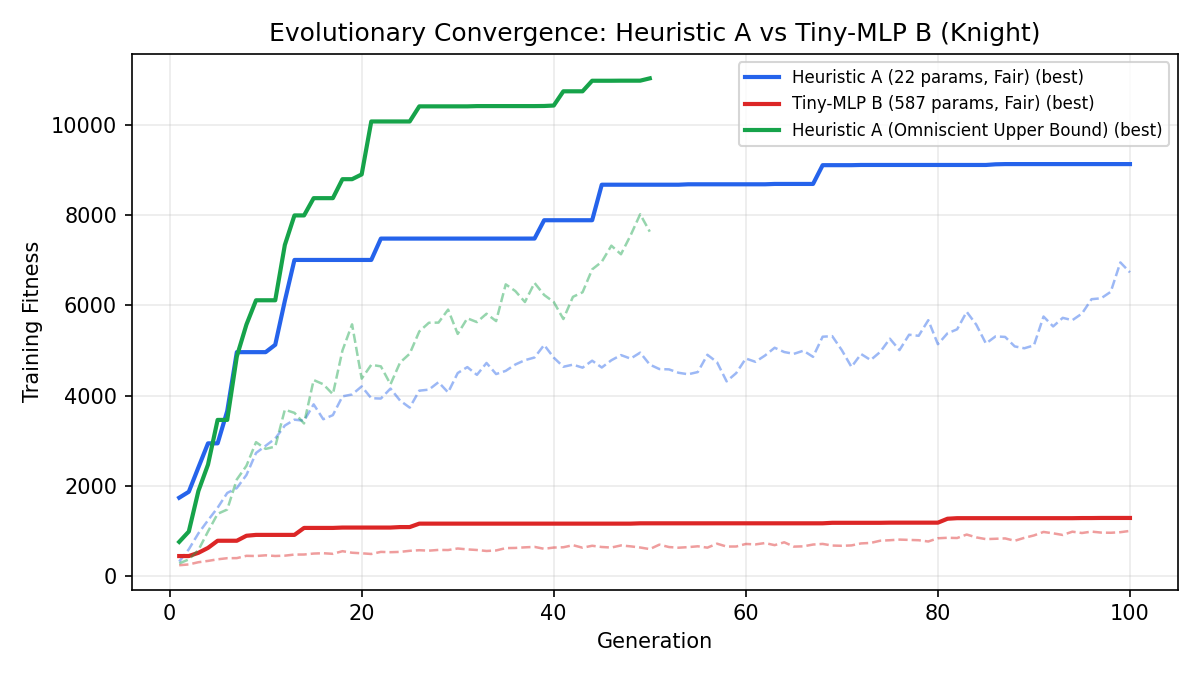
\includegraphics[width=\columnwidth]{figures/fitness_curves.png}
\caption{Evolutionary training fitness curves for three Knight runs: Fair Heuristic Deep, Fair Tiny-MLP Deep, and Omniscient Heuristic Medium.}
\label{fig:curves}
\end{figure}

\begin{figure}[t]
\centering
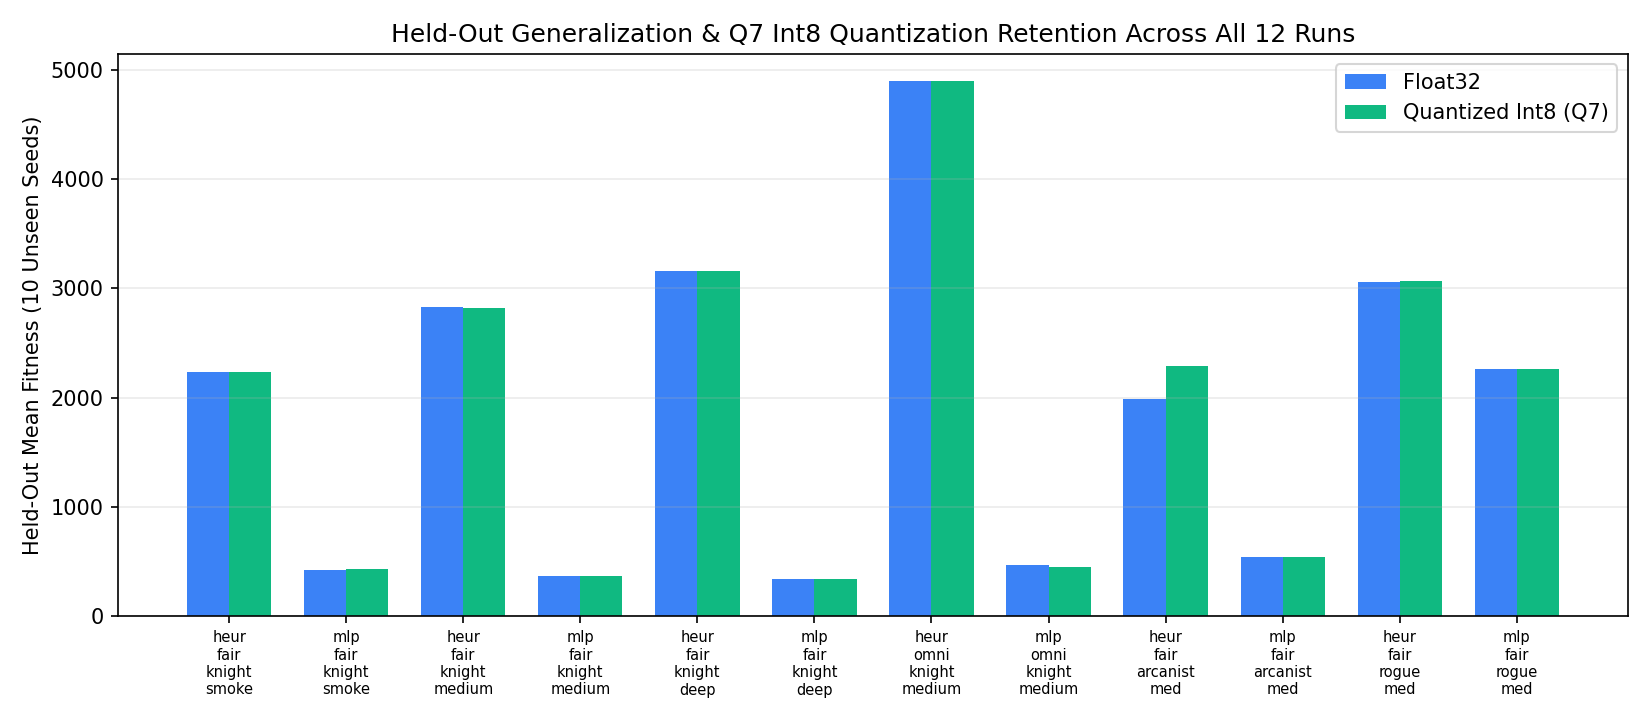
\includegraphics[width=\columnwidth]{figures/heldout_comparison.png}
\caption{Held-out 10-seed generalization comparing Float32 and Q7 \texttt{int8\_t} policies across all 12 benchmark experiments.}
\label{fig:heldout}
\end{figure}

\subsection{Key Empirical Findings}
\textbf{Budget Scaling:} Heuristic~A scales monotonically from Smoke (2,400 rollouts) to Medium (9,000) to Deep (36,000), raising Fair Knight held-out fitness from 2,233.3 $\to$ 2,833.4 $\to$ 3,156.7 ($+41.3\%$), held-out max floor from 4 $\to$ 5 $\to$ 6, and achieving a held-out Bone Warden boss kill in the Deep tier (3 boss kills and Floor~8 on training seeds). Tiny-MLP~B plateaus (415.6 $\to$ 366.7 $\to$ 336.6), indicating 587-D black-box search saturation.

\textbf{Heuristic~A vs.\ Tiny-MLP~B:} Across every matched setting, the 22-byte Heuristic~A outperforms the 587-byte Tiny-MLP~B in held-out Q7 fitness by 5.27$\times$ (Fair Knight Smoke), 7.70$\times$ (Fair Knight Medium), 9.37$\times$ (Fair Knight Deep), 10.95$\times$ (Omniscient Knight Medium), 4.23$\times$ (Fair Arcanist Medium), and 1.36$\times$ (Fair Rogue Medium), while using 26.7$\times$ less FRAM.

\textbf{Observability Ablation:} Removing Fog-of-War on Medium Knight increases Heuristic~A held-out Float fitness by $+73.1\%$ (2,833.4 $\to$ 4,904.5), mean floor from 2.2 $\to$ 3.6, and mean kills from 7.6 $\to$ 16.3 ($+114.5\%$). Tiny-MLP~B improves by $+27.6\%$ (366.7 $\to$ 468.0), confirming optimization rather than partial observability as its primary bottleneck.

\textbf{Class Specialists:} Under Medium Fair budgets, Heuristic~A Rogue achieves the highest held-out fitness (3,068.6 Q7) via $+1$ LOS and broader exploration (1,226.5 tiles), Knight reaches the deepest floors (max floor~5, 7.6--7.7 kills), and Arcanist (11~HP) exhibits lower generalization (1,985.9 Float / 2,291.4 Q7). Tiny-MLP~B Rogue reaches 2,261.4 (6.17$\times$ above MLP Knight) by triggering its starting Scroll of Mapping (1,071.4 explored tiles).

\textbf{Q7 Quantization Retention:} Across all 12 experiments, Q7 \texttt{int8\_t} achieves 101.08\% mean and 100.00\% median retention (Heuristic~A: 99.68\%--115.38\%; Tiny-MLP~B: 95.66\%--102.00\%). Retention above 100\% (e.g., \texttt{heur\_fair\_arcanist\_med} at 115.38\%) occurs when a Q7 tie-break alters a single discrete action and extends survival (\texttt{mean\_turns} 120.5 $\to$ 137.8).

\subsection{Live Hardware-in-the-Loop (HIL) Validation}
\texttt{ga/hil\_eval.py} evaluated both Deep Fair Knight Q7 \texttt{int8\_t} champions live over \texttt{COM4 @ 115200} baud against the physical MSP430FR5994 LaunchPad by reconstructing a Fair Fog-of-War \texttt{DungeonSim} proxy from live 80$\times$24 ANSI frames (\texttt{ga/results/hil\_knight\_deep.json} and \texttt{hil\_mlp\_deep.json}). On \texttt{SEED:9E6B} (\texttt{STONE CRYPT}), Heuristic~A completed 55 autonomous turns (22~gold, 1 \texttt{ESC[5n} DSR probe, 0~deaths) and Tiny-MLP~B completed 34 turns (47~gold, 2 \texttt{ESC[5n} probes, 0~deaths), both with 0 low-HP \texttt{BEL} alerts.

\section{On-Chip FRAM Deployment \& Resource Analysis}
Both Deep Fair Knight champions are exported to \texttt{app/ga\_weights.h} and compiled into \texttt{app/dungeon\_game.c} (\texttt{ga\_select\_action\_q7()}) with TI MSP430 Linker \texttt{v21.6.1}. Table~\ref{tab:mem} lists the exact post-Stage-4 footprint from \texttt{Debug/mspgame.map}.

\begin{table}[t]
\centering
\caption{Post-Stage-4 MSP430FR5994 Memory Footprint (Linker Map)}
\label{tab:mem}
\scriptsize
\begin{tabular}{@{}lcrrr@{}}
\toprule
Region / Symbol & Address & Used / Size & Capacity & Util. \\
\midrule
\texttt{RAM} (Main SRAM)         & \texttt{0x001c00} & 2,385 B & 4,096 B   & 58.23\% \\
\texttt{LEARAM} + \texttt{LEASTACK} & \texttt{0x002c00} & 0 B     & 4,096 B   &  0.00\% \\
\texttt{FRAM} (Lower)            & \texttt{0x004000} & 15,858 B & 49,024 B  & 32.35\% \\
\texttt{FRAM2} (Upper)           & \texttt{0x010000} & 29,808 B & 212,984 B & 14.00\% \\
\textbf{Total \texttt{FRAM+FRAM2}} & ---             & \textbf{45,666 B} & \textbf{262,008 B} & \textbf{17.43\%} \\
\midrule
AI Weights (\texttt{.const})     & \texttt{0x0077de} & 609 B   & 262,008 B &  0.23\% \\
\texttt{ga\_select\_action\_q7}  & \texttt{0x010000} & 3,668 B & 262,008 B &  1.40\% \\
\texttt{s\_ai\_hx}, \texttt{s\_ai\_hy} & \texttt{0x0022da} & 32 B    & 4,096 B   &  0.78\% \\
\bottomrule
\end{tabular}
\end{table}

Inference executes at most 242 integer MACs/turn (Approach~A) or 560 integer MACs/turn (Approach~B) with 0~B heap (\texttt{.sysmem} $= 0$). Inside \texttt{[4] AI DEMO}, the MCU steps autonomously every 500~ms; pressing \texttt{T} hot-swaps Heuristic~A (22~B) and Tiny-MLP~B (587~B) live on-chip, and \texttt{N} exits to Class Select.

\section{Discussion \& Limitations}
Our findings underscore that inductive bias dominates parameter count on ultra-low-power MCUs: 22 domain-aligned action weights outperform a 587-weight MLP by up to 10.95$\times$ under black-box evolution. Key limitations include: (1) train-to-held-out overfitting from 4--6 fixed training seeds per run, (2) a compact 16-entry SRAM visit ring buffer (32~B vs.\ 1,056~B full grid) retained after an audit restored 1:1 C/Python Q7 feature-encoding parity in \texttt{ga\_select\_action\_q7()}, and (3) 55-turn and 34-turn HIL runs bounded by real-time UART rendering cadence.

\section{Conclusion \& Future Work}
We demonstrated zero-float Q7 evolutionary policies running natively on a 16-bit TI MSP430FR5994 microcontroller. A 22-byte evolved heuristic reaches Floor~6 and defeats the Floor-5 boss on unseen seeds under Fair Fog-of-War (3,156.7 mean held-out fitness, 100.00\% Q7 retention) while coexisting with a 587-byte Tiny-MLP in just 609~B of FRAM. Future work will explore per-generation seed resampling and CMA-ES for MLP evolution, hardware-accelerated Q7 MACs via the untouched 4~KB MSP430 LEA, and class-specific 22-byte FRAM weight tables.

\section*{AI Usage \& Assistance Disclaimer}
This work was directed, architected, and verified by the human author (\texttt{joaogpd}). AI coding and research assistants were used transparently as engineering aids to assist with implementing the bit-faithful Python simulator, feature extractors, GA harness, and Q7 C-header exporter; automating the 12-experiment benchmark suite, figure generation, and HIL serial harness; integrating the Stage~4 Q7 inference engine into \texttt{app/dungeon\_game.c}; and drafting documentation and manuscript text. All architectural decisions, physical MSP430FR5994 LaunchPad validation, and verification of reported metrics were conducted under the human author's supervision, with every reported value derived strictly from logged JSON/map outputs and repository source files.

\begin{thebibliography}{6}
\bibitem{ti_ds} Texas Instruments, \emph{MSP430FR599x, MSP430FR596x Mixed-Signal Microcontrollers Datasheet (SLASE54)}, 2021.
\bibitem{ti_ug} Texas Instruments, \emph{MSP430FR58xx, MSP430FR59xx, and MSP430FR6xx Family User's Guide (SLAU367)}, 2020.
\bibitem{goldberg} D.~E. Goldberg, \emph{Genetic Algorithms in Search, Optimization, and Machine Learning}. Addison-Wesley, 1989.
\bibitem{salimans} T.~Salimans, J.~Ho, X.~Chen, S.~Sidor, and I.~Sutskever, ``Evolution strategies as a scalable alternative to reinforcement learning,'' \emph{arXiv:1703.03864}, 2017.
\bibitem{jacob} B.~Jacob \emph{et al.}, ``Quantization and training of neural networks for efficient integer-arithmetic-only inference,'' in \emph{Proc.\ IEEE/CVF CVPR}, 2018, pp.~2704--2713.
\bibitem{bresenham} J.~Bresenham, ``Algorithm for computer control of a digital plotter,'' \emph{IBM Systems Journal}, vol.~4, no.~1, pp.~25--30, 1965.
\end{thebibliography}

\end{document}
